\documentclass[12pt]{article}
\usepackage[utf8]{inputenc}
\usepackage[margin=1in]{geometry}
\usepackage{amsmath}\usepackage{amssymb}\usepackage{multicol}\usepackage{enumitem}
\usepackage{pgfplots}\pgfplotsset{compat=1.17}
\setlength{\parindent}{0pt}
\begin{document}

\fbox{\parbox{0.97\linewidth}{\small\textbf{Final answers} (record here --- graded on the answer; show your work):\\[6pt]1.~\underline{\hspace{1.5cm}}\quad 2.~\underline{\hspace{1.5cm}}\quad 3.~\underline{\hspace{1.5cm}}\quad 4.~\underline{\hspace{1.5cm}}\quad 5.~\underline{\hspace{1.5cm}}\quad 6.~\underline{\hspace{1.5cm}}\quad 7.~\underline{\hspace{1.5cm}}\quad 8.~\underline{\hspace{1.5cm}}\quad 9.~\underline{\hspace{1.5cm}}\quad 10.~\underline{\hspace{1.5cm}}\quad 11.~\underline{\hspace{1.5cm}}\quad 12.~\underline{\hspace{1.5cm}}}}
\vspace{0.35cm}

\begin{center}{\Large \textbf{Warm-Up: Shifts}}\end{center}\vspace{0.2cm}
% Warm-Up: Shifts
\textbf{Example (Warm-Up: Shifts):}

$y=x^2-6$ shifts $y=x^2$ down 6 units; vertex $(0,-6)$.

\vspace{0.2cm}\hrule\vspace{0.35cm}
\textbf{Directions: Describe the shift and state the vertex for each function.}

\begin{multicols}{2}
\begin{enumerate}[label=\textbf{\arabic*.}, start=1, itemsep=1.3cm]
  \item $\displaystyle y=x^2+4$
  \item $\displaystyle y=(x-3)^2$
  \item $\displaystyle y=(x+5)^2$
  \item $\displaystyle y=x^2-2$
\end{enumerate}
\end{multicols}
\vspace{0.25cm}\hrule\vspace{0.35cm}

\begin{center}{\Large \textbf{Reflections and Stretches}}\end{center}\vspace{0.2cm}
% Reflections and Stretches
\textbf{Example (Reflections and Stretches):}

$y=-3x^2$ reflects $y=x^2$ over the x-axis and stretches it (narrower) by a factor of 3.

\vspace{0.2cm}\hrule\vspace{0.35cm}
\textbf{Directions: Describe the reflection and/or stretch/compression for each function.}

\begin{multicols}{2}
\begin{enumerate}[label=\textbf{\arabic*.}, start=5, itemsep=2cm]
  \item $\displaystyle y=-x^2$
  \item $\displaystyle y=4x^2$
  \item $\displaystyle y=\frac{1}{4}x^2$
  \item $\displaystyle y=-\frac{1}{2}x^2$
\end{enumerate}
\end{multicols}
\vspace{0.25cm}\hrule\vspace{0.35cm}

\begin{center}{\Large \textbf{Combined Transformations}}\end{center}\vspace{0.2cm}
% Combined Transformations
\textbf{Example (Combined Transformations):}

$y=-2(x-1)^2+4$: shift right 1, reflect over x-axis, stretch narrower by 2, shift up 4; vertex $(1,4)$.

\begin{center}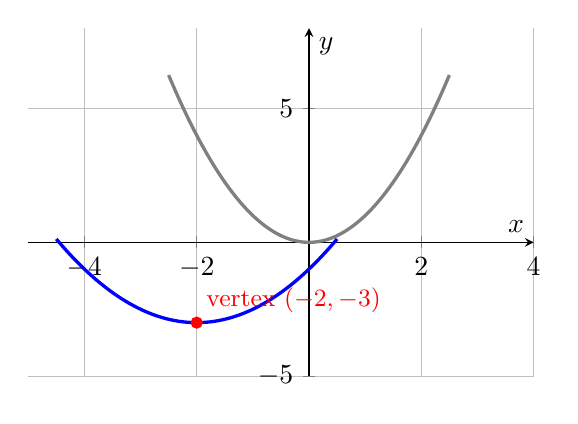
\begin{tikzpicture}
\begin{axis}[axis lines=middle,xlabel=$x$,ylabel=$y$,xmin=-5,xmax=4,ymin=-5,ymax=8,width=8cm,height=6cm,grid=both,samples=80]
\addplot[very thick,gray,domain=-2.5:2.5]{x^2};
\addplot[very thick,blue,domain=-4.5:0.5]{0.5*(x+2)^2-3};
\addplot[only marks,mark=*,red] coordinates {(-2,-3)};
\node[above right,red,font=\small] at (axis cs:-2,-3) {vertex $(-2,-3)$};
\end{axis}\end{tikzpicture}\end{center}
{\small\centering $y=x^2$ (gray) transformed into $y=\frac{1}{2}(x+2)^2-3$ (blue).\par}
\vspace{0.2cm}\hrule\vspace{0.35cm}
\textbf{Directions: Describe all transformations (shift, reflection, stretch/compression) and state the final vertex.}

\begin{multicols}{2}
\begin{enumerate}[label=\textbf{\arabic*.}, start=9, itemsep=3cm]
  \item $y=\frac{1}{2}(x+2)^2-3$ (use the graph above to confirm your description)
  \item $\displaystyle y=3(x-4)^2-1$
  \item $\displaystyle y=-\frac{1}{3}(x+2)^2+5$
\end{enumerate}
\end{multicols}

\vspace{0.2cm}\hrule\vspace{0.3cm}
\textbf{Challenge} (same sheet):\\[4pt]
\begin{enumerate}[label=\textbf{\arabic*.}, start=12, itemsep=2.2cm]
  \item Describe the transformations, in order, that turn $y=x^2$ into $y=-4(x+3)^2-7$.
\end{enumerate}

\newpage

\begin{center}{\Large \textbf{Answer Key --- fully worked}}\end{center}
\vspace{0.25cm}
\textbf{Procedure:} Start from the parent function $y=x^2$.; Identify $h$: shift left if the equation has $(x+h)$, right if $(x-h)$.; Identify $k$: shift up if positive, down if negative.; Check the sign of $a$: negative means reflect over the x-axis.; Check the size of $|a|$: greater than 1 means narrower (stretch), between 0 and 1 means wider (compression).; Combine all transformations to state the final vertex and shape..\\[8pt]
\begin{enumerate}[label=\textbf{\arabic*.},itemsep=7pt]
  \item Shifts up 4; vertex $(0,4)$.
  \item Shifts right 3; vertex $(3,0)$.
  \item Shifts left 5; vertex $(-5,0)$.
  \item Shifts down 2; vertex $(0,-2)$.
  \item Reflects over the x-axis; no stretch (a=-1).
  \item Stretches narrower by a factor of 4; no reflection.
  \item Compresses wider by a factor of $\frac{1}{4}$; no reflection.
  \item Reflects over the x-axis and compresses wider by a factor of $\frac{1}{2}$.
  \item Shift left 2, compress wider by $\frac{1}{2}$ (no reflection), shift down 3; vertex $(-2,-3)$ -- matches the graph shown.
  \item Shift right 4, stretch narrower by 3 (no reflection), shift down 1; vertex $(4,-1)$.
  \item Shift left 2, reflect over the x-axis and compress wider by $\frac{1}{3}$, shift up 5; vertex $(-2,5)$.
  \item In order from the parent $y=x^2$: (1) $(x+3)$ shifts the graph left 3 units; (2) the negative sign reflects it over the x-axis; (3) $|a|=4>1$ stretches it narrower by a factor of 4; (4) the $-7$ shifts it down 7 units. Final vertex: $(-3,-7)$, opening down.
\end{enumerate}

\end{document}